\chapter{The Basics}

\section{Data Design and Abstraction}

Designing a friendly HTTP API means abstracting the intricate business-logic and data your service uses into the four basic CRUD concepts (\emph{Create}, \emph{Read}, \emph{Update}, \emph{Delete}). Your application may perform many complex actions behind the scenes such as sending a text message or resizing an image or moving a file, but if you do enough planning and abstraction, everything can be represented as CRUD.

Architecting your API begins earlier than you may think; first you need to decide how your data will be stored and how your service/application functions. If you're practicing \href{http://blog.pop.co/post/67465239611/why-we-chose-api-first-development}{API-First Development} \cite{APIFIRST} this is all part of the process. However, if you're bolting an API onto an existing project, you will have more abstraction to take care of.

In an idealized, overly-simple service, a Collection can represent a database table, and a Resource can represent a row within that table. As real-world practice will show this is rarely the case, especially if the existing data design is overly complex. It is important that you don't overwhelm third-party developers with complex application data, otherwise they won't want to use your API.

There will be parts of your service which you \emph{should not} expose via API at all. A common example is that many APIs will not allow Consumers to create or delete user accounts, or data shared between many accounts.

Sometimes multiple tables will be represented as a single resource (\texttt{JOIN} statements come in handy here). You might even find that one table should have multiple resources (although, you may have made some poor database design decisions if this is the case).

\subsection{Examples of Abstraction}

For both of these examples of abstraction, we'll make use of the same fictional service. This service sends messages to different users, and messages can either be sent as a text message or an email. The chosen method depends on the preference of the particular user.

Don't worry too much about the technical parts of the examples as we'll cover them with more detail in a later chapter. For now, just think of them as simple function calls with inputs and outputs.

\subsubsection{Good Abstraction}

Here's a clean and simple approach for sending a notification.

\paragraph{\textbf{Creating a Notification}}

\begin{verbatim}
POST /notifications

{
  "user_id": "12",
  "message": "Hello World"
}

{
  "id": "1000",
  "user_id": "12",
  "message": "Hello World",
  "medium": "email",
  "created": "2013-01-06T21:02:00Z"
}
\end{verbatim}

In this example we use a single endpoint for sending a notification to a user. The first JSON document is the request and the second is the response. This endpoint is called \texttt{notifications}, and the Consumer interacts by creating new notification objects. When the Consumer wishes to notify a user, it is conceptually creating a new notification object, thereby abstracting the concept of performing an action with creating an object.

An important concept of this example is that the business-logic of determining which method of contacting a user is abstracted away from the Consumer entirely, hence the lack of an endpoint for getting the users notification preference. In the background, the Server is taking the appropriate action and hiding it from the Consumer.

In the example response, we do have a \texttt{medium} attribute which represents the method of notifying the user, but that can be omitted depending on if your Consumers need to know this information (perhaps their application has a dashboard which mentions the last time a text/email was sent, and the verbiage should be correct).

\subsubsection{Bad Abstraction}

This example will include numerous shortcomings, and is an easy approach to take by the novice HTTP API architect.

\paragraph{\textbf{Getting User Preference}}

\begin{verbatim}
GET /get_user_preferences/12

{
  "notification_preference": 1
}
\end{verbatim}

This first API Endpoint is called \texttt{get\_user\_preferences}, and is called by passing in the ID of the user whose preference we are looking up (shown here as \texttt{12}). The name of an Endpoint should be a simple noun (or compound nouns). It should not include the action (verb) being performed (in this case \texttt{get}). The reason one should use a simple noun is because this removes ambiguity and tells the Consumer what the ID represents. Does the \texttt{12} represent user \texttt{12}? Or perhaps some user-preference concept which might not correlate 1:1 to a user object?

Another problem with this example is the response contains the integer \texttt{1}. Internally to this fictional service there are some constants where \texttt{1} refers to sending a text, and \texttt{2} refers to sending an email. Even if these values are disclosed in the API documentation, a third-party developer is not going to remember what they represent. Each time they look up what the values mean they are losing productivity.

Yet another problem is that there's an API Endpoint dedicated specifically to getting a user preference. In general, you want to reduce the number of Endpoints in your API, and focus on making each one serve the Consumer better. Data like this could have been merged with another endpoint for getting a user object, for example.

\paragraph{\textbf{Sending a Text or Email (Two Endpoints)}}

\begin{verbatim}
POST /users/12/send_{medium}

{
  "message": "Hello World",
  "sent": "2013-01-06T21:02:00Z"
}
\end{verbatim}

These second and third endpoints (assuming \texttt{\{medium\}} can represent \texttt{email} or \texttt{text}) have the same problem as the previous endpoint wherein the action is part of the URL (in this case \texttt{send}). These endpoints don't represent data, as the previous one did, they specifically represent an action. Building APIs with these actionable endpoints is a common mistake among developers intending to build an HTTP API.

Another issue with this example is that the business-logic for determining which method of notification to use is left for the Consumer to decide! Sure, the Consumer can make a request to get the users preference, but what if they intentionally ignore it? Or suppose the Consumer caches the preference and it becomes outdated? Either way users are bound to get notified in a manner they didn't choose.

Whenever you find yourself creating two endpoints with the same request inputs and response outputs, there may be a problem with abstraction and the two may be better off combined into one endpoint.

Finally, there is no way to look up previous instances of notifications that have been sent to a user. While another Endpoint could have been created for looking up notification logs, it would likely be ad-hoc or inconsistent with existing Endpoints.

\subsection{Real World Examples}

Let's look at some real-world examples of how popular APIs do their data abstraction.

\subsubsection{GitHub: An Ideal Example}

The current GitHub v3 API \cite{GITHUBAPI} is a beautiful example of a properly-abstracted HTTP API. Each of the popular HTTP verbs are used where applicable. Endpoints don't have verbs in the name. Interacting with an endpoint feels much like one is working with a representation of an object, instead of performing actions.

An example of a good endpoint is \texttt{GET /repos/\{user\_id\}/\{repo\_id\}/notifications}. This is obviously the endpoint used for getting a list of notifications of a particular repository. The \texttt{\{user\_id\}/\{repo\_id\}} convention for referring to a repository is one understood by most users of GitHub (repository names aren't globally unique, only unique to a particular user). The only thing that could be improved may be to not shorten \texttt{repositories} to \texttt{repos} and \texttt{organizations} to \texttt{orgs} in the names of endpoints, although \texttt{repo} is well understood.

\subsubsection{Twitter: A Flawed Example}

The current Twitter v1.1 API \cite{TWITTERAPI} has some abstraction shortcomings with their data and business-logic, as far as being an HTTP API is concerned. The API only makes use of the GET and POST methods for interacting with data. Due to this shortcoming, most endpoint names are a pair of noun and verbs.

One such example is \texttt{POST /statuses/destroy/\{status\_id\}}, used for deleting a status. A cleaner version of this endpoint would be \texttt{DELETE /statuses/\{status\_id\}}. Also worth noting is the differentiation of \texttt{POST /statuses/update\_with\_media} and \texttt{POST /statuses/update}. Both of these endpoints are used for creating a new tweet, however the prior allows for the attachment of media. These two endpoints should be combined into a single \texttt{POST /statuses}, with the media related attributes being optional.

These endpoints are also an example of a bad nomenclature. Users of Twitter don't think of using the service as \emph{updating their status}, they think of it as \emph{tweeting}. This is something that may have changed throughout the lifetime of the service, and if so would be a good candidate to change between API versions. The Collection used by the aforementioned Endpoints would therefor be better named \texttt{tweets}.


\section{Anatomy of an HTTP Message}

Since HTTP is the protocol we're using to build our API, let's examine some raw HTTP messages. It's surprising how many developers who have been building websites for years don't know what an HTTP message looks like! When the Consumer sends a request to the Server, it provides a Request-Line and a set of Key/Value pairs called headers. For POST, PUT, and PATCH requests it also provides two newlines and then the the request body. All This information is sent in the same HTTP request (although this request can be broken up into multiple network packets if the message is large enough).

The Server then replies in a similar format, first with a Status-Line and headers, and typically two newlines followed by a body (the body is technically optional, as you'll find out later). HTTP is very much a request/response protocol; there is no \emph{push} support (the Server does not send data to the Consumer unprovoked). To do that you would need to use a different protocol such as Websockets.

\subsection{HTTP Request}

\begin{verbatim}
POST /v1/animal HTTP/1.1
Host: api.example.org
Accept: application/json
Content-Type: application/json
Content-Length: 24

{
  "name": "Gir",
  "animal_type": "12"
}
\end{verbatim}

\subsection{HTTP Response}

\begin{verbatim}
HTTP/1.1 200 OK
Date: Wed, 18 Dec 2013 06:08:22 GMT
Content-Type: application/json
Access-Control-Max-Age: 1728000
Cache-Control: no-cache

{
  "id": "12",
  "created": "2013-12-18T06:08:22Z",
  "modified": null,
  "name": "Gir",
  "animal_type": "12"
}
\end{verbatim}

\subsection{Debugging HTTP Traffic}

\href{http://getpostman.com/}{Postman} (a Google Chrome extension) is an excellent tool for interacting with an HTTP API. As seen in Figure ~\ref{fig:postman}, Postman provides a powerful yet easy-to-use interface for building API requests, as well as debugging the content of API responses. It also provides many advanced features regarding authentication (which we'll cover in later chapters).

\begin{figure}[ht!]
\centering
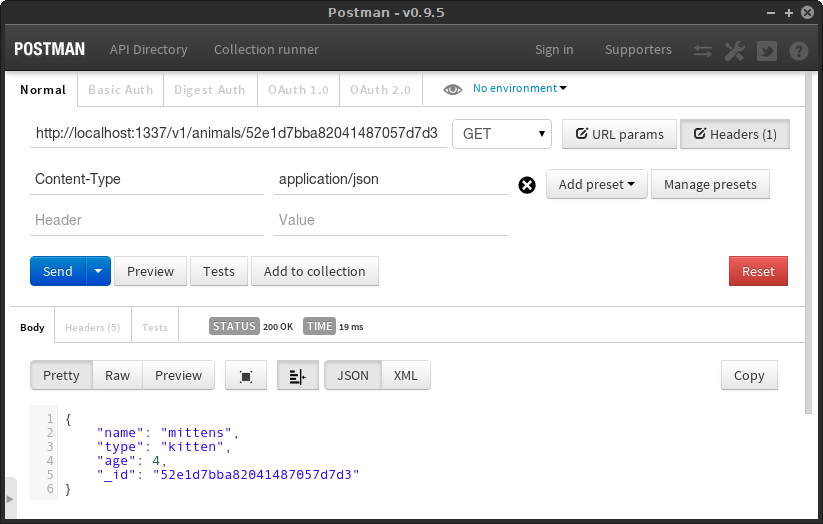
\includegraphics[width=3.8in]{images/postman.png}
\caption{Postman Screenshot}
\label{fig:postman}
\end{figure}

While designing and debugging your API you will sometimes need to debug packets at a lower level than HTTP. A powerful tool for doing this is \href{https://www.wireshark.org}{Wireshark}. You will also want to use a web framework and server which allows you to read and change as many headers as possible.

Figure ~\ref{fig:wireshark} is an example of a complex HTTP request from a form submission on a website. Notice all of the data sent back and forth via HTTP headers. The headers passed around by browsers and web servers is often more chaotic and noisy than what an API Consumer and Server will send.

\begin{figure}[ht!]
\centering
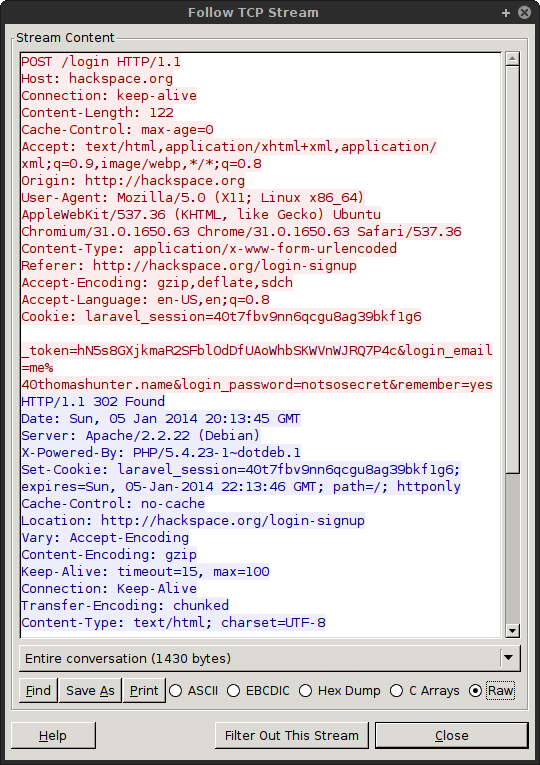
\includegraphics[height=3in]{images/wireshark.png}
\caption{Wireshark Screenshot}
\label{fig:wireshark}
\end{figure}


\section{API Entrypoint}

The root location of your API is important, believe it or not. When a third-party developer (aka \emph{code archaeologist}) inherits a project using your API and needs to build new features, they may not know about your service at all. Perhaps all they know is a list of URLs which the Consumer communicates with. It's important that the root entry point into your API is as simple as possible, as a long complex URL will appear daunting and can turn developers away.

\subsection{Choosing an Entrypoint}

Here are two common URL schemes that developers use when building an API. These are also sometimes called API entry points.

\begin{itemize}
\item \texttt{https://api.example.com/*} -- \emph{Preferred}
\item \texttt{https://example.org/api/*} -- \emph{Security Implications}
\end{itemize}

First, notice the HTTPS prefix. If API communication is sent unencrypted over the Internet, any third-party along the way is able to eavesdrop. This could include reading sensitive API data, and depending on the chosen authentication method, could allow third-parties to make requests on behalf of the user.

If your application is huge, or you anticipate it becoming huge, putting the API on a dedicated subdomain (in this case \texttt{api.}) is a must. This will allow for more scalability options in the future. It can also be useful for controlling what cookie data can be shared between the content website and the API.

If you anticipate your API will never become large, or you want to build a simple application (e.g. you want to host the website AND API from the same framework), or if your API is entirely anonymous or read-only, placing your API beneath a URL segment at the root of the domain (e.g. \texttt{/api/}) will also work, however it is not a great idea. More considerations will need to be made regarding security, and more potential vulnerabilities can arise. For example, if an XSS vulnerability is discovered on the main website, credentials which might not otherwise be exposed can now be hijacked by a devious third-party.

Do not use a different Top Level Domain (TLD) for hosting your API than for hosting your website. This may sound tempting, as your main domain could be \textbf{example.com}, and your API and developer documentation be entirely located on the trendy \textbf{example.io}. However there is no logical relationship between these two domains as an adversary could have purchased \textbf{example.io}, posing as a legitimate counterpart to \textbf{example.com}. Also, the \emph{code archaeologist} might only have knowledge of one domain and not the other. Finally, if you \emph{do} want to share cookies between the two domains (e.g. an authenticated user on \textbf{example.com} can be automatically logged into the developer site) it cannot be done as easily with two separate TLDs than with a subdomain or even a subdirectory.

\subsection{Content Located at the Root}

It's beneficial to Consumers to have content at the root of your API. For example, accessing the root of GitHub's API returns a listing of endpoints. Personally I'm a fan of having the root URL give information which a lost developer would find useful, like how to get to the developer documentation.

Here's a truncated list of the content provided by the \href{https://api.github.com/}{GitHub API Entrypoint}.

\begin{verbatim}
{
  "current_user_url": "https://api.github.com/user",
  "authorizations_url":
    "https://api.github.com/authorizations",
  "emails_url": "https://api.github.com/user/emails",
  "starred_url":
    "https://api.github.com/user/starred{/owner}{/repo}",
  ...
}
\end{verbatim}

The syntax used to describe these URLs is called a URI Template and is a human-readable and machine-parsable standard for describing URLs. This is a great way to convey URLs in both your API documentation, as well as the API responses themselves.

\begin{quote}
A URI Template is a compact sequence of characters for describing a range of Uniform Resource Identifiers through variable expansion. \cite{RFC6570}
\end{quote}

Information about the currently-authenticated user can also be placed in the root of the API. As an example, either the user ID or URL to the user would make a great candidate. If you take a similar approach to what GitHub does, one of the keys could be \texttt{current\_user}, and the value could be a URL to the \texttt{users} endpoint pre-populated with the current users \texttt{user\_id}.

It may be tempting to create an endpoint called \texttt{/user} or \texttt{/users/me} for accessing information about the current user, but these would contradict the existing URL patterns the rest of the API adheres to.
